\subsection{UC2 - Scelta della visualizzazione}
\label{uc2}

    \begin{figure}[htbp]
        \centering
        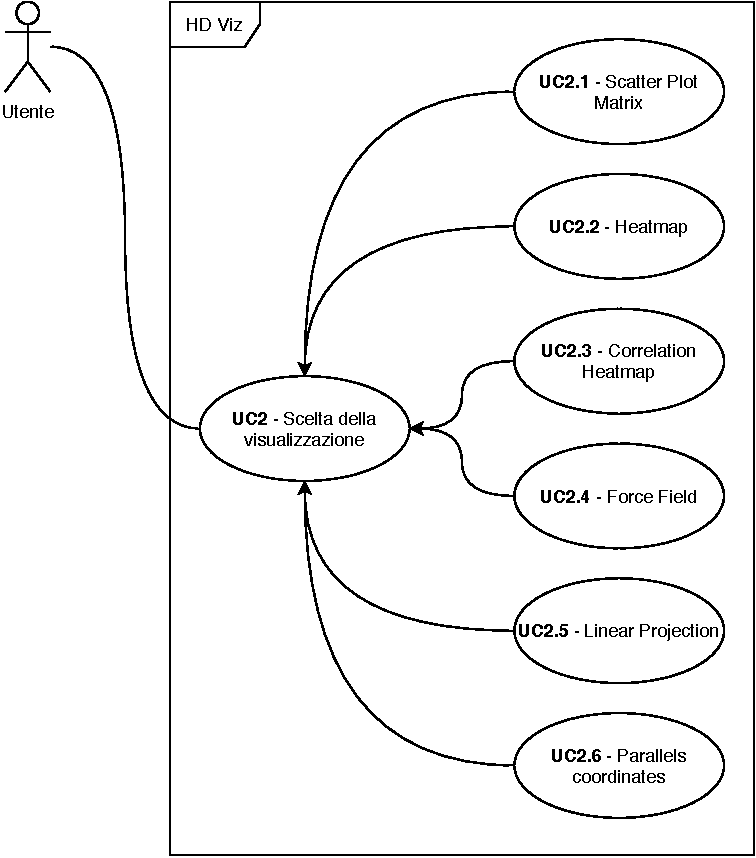
\includegraphics[width=0.75\textwidth]{source/sections/casi-uso/diagrams/uc2.pdf}
        \caption{UC2 - Scelta della visualizzazione}
        \label{fig:uc2}
    \end{figure}

    % \includegraphics{}
    \begin{itemize}
    \item \textbf{Attore}: utente;
    \item \textbf{Descrizione}: l'utente all'interno dell'applicazione sceglie la visualizzazione che vuole ottenere;
    \item \textbf{Precondizione}:
    \begin{itemize}
        \item il sistema è funzionante e raggiungibile;
        \item l'utente accede alla pagina dell'applicazione.
    \end{itemize}
    \item \textbf{Postcondizione}: l'utente ha scelto quale visualizzazione vuole ottenere;
    \item \textbf{Scenario Principale}: 
        \begin{enumerate}
            \item l'utente seleziona la visualizzazione tra quelle disponibili.
        \end{enumerate}  
    \item \textbf{Generalizzazioni}:
        \begin{enumerate}
            \item l'utente seleziona una delle seguenti visualizzazioni:
                \begin{enumerate}
                    \item Scatter Plot Matrix (\hyperref[uc2.1]{UC2.1});
                    \item Heatmap (\hyperref[uc2.2]{UC2.2});
                    \item Correlation Heatmap (\hyperref[uc2.3]{UC2.3});
                    \item Force Field (\hyperref[uc2.4]{UC2.4});
                    \item Linear Projection (\hyperref[uc2.5]{UC2.5});
                    \item Parallel Coordinates (\hyperref[uc2.6]{UC2.6}).
                \end{enumerate}
        \end{enumerate}  
    \end{itemize}
    
    %%%
    \subsubsection{UC2.1 - Scatter Plot Matrix}
    \label{uc2.1}
    
    \begin{itemize}
    \item \textbf{Attore}: utente;
    \item \textbf{Descrizione}: l'utente sceglie la visualizzazione \emph{Scatter Plot Matrix};
    \item \textbf{Precondizione}:
    \begin{itemize}
        \item il sistema è funzionante e raggiungibile;
        \item l'utente accede alla pagina dell'applicazione.
    \end{itemize}
    \item \textbf{Postcondizione}: l'utente sceglie Scatter Plot Matrix come visualizzazione;
    \item \textbf{Scenario Principale}: 
        \begin{enumerate}
            \item l'utente sceglie Scatter Plot Matrix come visualizzazione.
        \end{enumerate}
    \end{itemize}
    
    %%%
    \subsubsection{UC2.2 - Heatmap}
    \label{uc2.2}
    
    \begin{itemize}
    \item \textbf{Attore}: utente;
    \item \textbf{Descrizione}: l'utente sceglie la visualizzazione \emph{Heatmap};
    \item \textbf{Precondizione}:
    \begin{itemize}
        \item il sistema è funzionante e raggiungibile;
        \item l'utente accede alla pagina dell'applicazione.
    \end{itemize}
    \item \textbf{Postcondizione}: l'utente sceglie Heatmap come visualizzazione;
    \item \textbf{Scenario Principale}: 
        \begin{enumerate}
            \item l'utente sceglie Heatmap come visualizzazione.
        \end{enumerate}
    \end{itemize}
    
    %%%
    \subsubsection{UC2.3 - Correlation Heatmap}
    \label{uc2.3}
    
    \begin{itemize}
    \item \textbf{Attore}: utente;
    \item \textbf{Descrizione}: l'utente sceglie la visualizzazione \emph{Correlation Heatmap};
    \item \textbf{Precondizione}:
    \begin{itemize}
        \item il sistema è funzionante e raggiungibile;
        \item l'utente accede alla pagina dell'applicazione.
    \end{itemize}
    \item \textbf{Postcondizione}: l'utente sceglie Correlation Heatmap come visualizzazione;
    \item \textbf{Scenario Principale}: 
        \begin{enumerate}
            \item l'utente sceglie Correlation Heatmap come visualizzazione.
        \end{enumerate}
    \end{itemize}
    
    %%%
    \subsubsection{UC2.4 - Force Field}
    \label{uc2.4}
    
    \begin{itemize}
    \item \textbf{Attore}: utente
    \item \textbf{Descrizione}: l'utente sceglie la visualizzazione \emph{Force Field};
    \item \textbf{Precondizione}:
    \begin{itemize}
        \item il sistema è funzionante e raggiungibile;
        \item l'utente accede alla pagina dell'applicazione.
    \end{itemize}
    \item \textbf{Postcondizione}: l'utente sceglie Force Field come visualizzazione;
    \item \textbf{Scenario Principale}: 
        \begin{enumerate}
            \item l'utente sceglie Force Field come visualizzazione.
        \end{enumerate}
    \end{itemize}
    
    %%%
    \subsubsection{UC2.5 - Linear Projection}
    \label{uc2.5}
    
    \begin{itemize}
    \item \textbf{Attore}: utente;
    \item \textbf{Descrizione}: l'utente sceglie la visualizzazione \emph{Linear Projection};
    \item \textbf{Precondizione}:
    \begin{itemize}
        \item il sistema è funzionante e raggiungibile;
        \item l'utente accede alla pagina dell'applicazione.
    \end{itemize}
    \item \textbf{Postcondizione}: l'utente sceglie Linear Projection come visualizzazione;
    \item \textbf{Scenario Principale}: 
        \begin{enumerate}
            \item l'utente sceglie Linear Projection come visualizzazione.
        \end{enumerate}
    \end{itemize}
    
    %%%
    \subsubsection{UC2.6 - Parallel Coordinates}
    \label{uc2.6}
    
    \begin{itemize}
    \item \textbf{Attore}: utente;
    \item \textbf{Descrizione}: l'utente sceglie la visualizzazione \emph{Parallel Coordinates};
    \item \textbf{Precondizione}:
    \begin{itemize}
        \item il sistema è funzionante e raggiungibile;
        \item l'utente accede alla pagina dell'applicazione.
    \end{itemize}
    \item \textbf{Postcondizione}: l'utente sceglie Parallel Coordinates come visualizzazione;
    \item \textbf{Scenario Principale}: 
        \begin{enumerate}
            \item l'utente sceglie Parallel Coordinates come visualizzazione.
        \end{enumerate}
    \end{itemize}
    
  
